\chapter{Flexbox e Grid}
\label{cap:flexbox_grid}

\section{Introduzione ai Layout Moderni}

Prima di Flexbox e Grid, i layout CSS erano implementati con tecniche complesse e poco intuitive come float, position e table-cell, rendendo il codice difficile da mantenere. I layout moderni CSS3 risolvono questi problemi in modo elegante e intuitivo. Con Flexbox, puoi creare layout monodimensionali che si adattano facilmente a riga o colonna. CSS Grid introduce il concetto di layout bidimensionale, permettendoti di controllare contemporaneamente righe e colonne. Questi strumenti forniscono allineamento intuitivo, rendendo il centramento verticale e orizzontale semplice e naturale, un compito che prima era notoriamente difficile. Offrono anche responsività automatica, consentendo ai tuoi layout di adattarsi automaticamente a diverse dimensioni di schermo senza codice aggiuntivo. Un'altra caratteristica potente è l'ordinamento visuale, che permette di cambiare l'ordine di visualizzazione degli elementi senza modificare l'HTML sottostante, migliorando la flessibilità del design.

\begin{nota}
Flexbox e Grid non sono in competizione: sono complementari. Usa Flexbox per componenti (navbar, card) e Grid per layout di pagina completi.
\end{nota}

\section{Flexbox}

\subsection{Concetti Fondamentali}

Flexbox (Flexible Box Layout) è un modello di layout monodimensionale che permette di distribuire spazio e allineare elementi lungo un \textbf{asse principale} (main axis) e un \textbf{asse trasversale} (cross axis).

\subsubsection{Terminologia Flexbox}

\begin{description}
  \item[Flex container] Elemento genitore con \texttt{display: flex} o \texttt{display: inline-flex}
  \item[Flex items] Elementi figli diretti del container
  \item[Main axis] Asse principale (orizzontale con row, verticale con column)
  \item[Cross axis] Asse perpendicolare al main axis
  \item[Main start/end] Inizio e fine dell'asse principale
  \item[Cross start/end] Inizio e fine dell'asse trasversale
\end{description}

\subsubsection{Diagramma Assi Flexbox}

\begin{center}
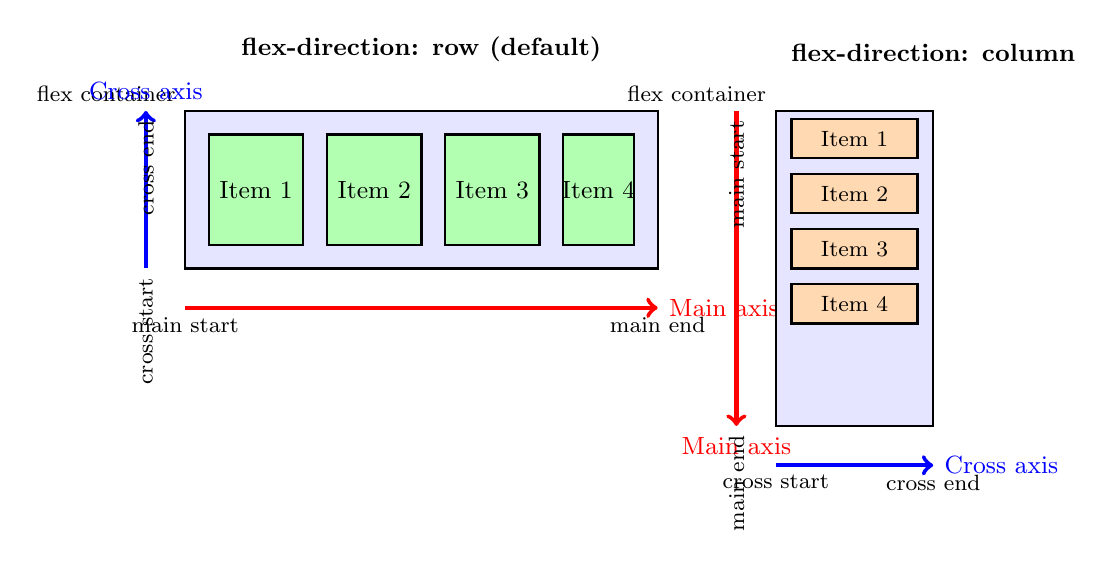
\begin{tikzpicture}[scale=1.0]
    % Flex container row
    \node[above, font=\small\bfseries] at (3,4.5) {flex-direction: row (default)};
    \draw[thick, fill=blue!10] (0,2) rectangle (6,4);
    \node[above left, font=\footnotesize] at (0,4) {flex container};

    % Flex items
    \draw[thick, fill=green!30] (0.3,2.3) rectangle (1.5,3.7);
    \node[font=\small] at (0.9,3) {Item 1};

    \draw[thick, fill=green!30] (1.8,2.3) rectangle (3.0,3.7);
    \node[font=\small] at (2.4,3) {Item 2};

    \draw[thick, fill=green!30] (3.3,2.3) rectangle (4.5,3.7);
    \node[font=\small] at (3.9,3) {Item 3};

    \draw[thick, fill=green!30] (4.8,2.3) rectangle (5.7,3.7);
    \node[font=\small] at (5.25,3) {Item 4};

    % Main axis (orizzontale)
    \draw[->, ultra thick, red] (0,1.5) -- (6,1.5) node[right, font=\small] {Main axis};
    \node[below, font=\footnotesize] at (0,1.5) {main start};
    \node[below, font=\footnotesize] at (6,1.5) {main end};

    % Cross axis (verticale)
    \draw[->, ultra thick, blue] (-0.5,2) -- (-0.5,4) node[above, font=\small] {Cross axis};
    \node[left, font=\footnotesize, rotate=90] at (-0.5,2) {cross start};
    \node[left, font=\footnotesize, rotate=90] at (-0.5,4) {cross end};

    % Flex container column
    \node[above, font=\small\bfseries] at (9.5,4.5) {flex-direction: column};
    \draw[thick, fill=blue!10] (7.5,0) rectangle (9.5,4);
    \node[above left, font=\footnotesize] at (7.5,4) {flex container};

    % Flex items verticali
    \draw[thick, fill=orange!30] (7.7,3.4) rectangle (9.3,3.9);
    \node[font=\footnotesize] at (8.5,3.65) {Item 1};

    \draw[thick, fill=orange!30] (7.7,2.7) rectangle (9.3,3.2);
    \node[font=\footnotesize] at (8.5,2.95) {Item 2};

    \draw[thick, fill=orange!30] (7.7,2.0) rectangle (9.3,2.5);
    \node[font=\footnotesize] at (8.5,2.25) {Item 3};

    \draw[thick, fill=orange!30] (7.7,1.3) rectangle (9.3,1.8);
    \node[font=\footnotesize] at (8.5,1.55) {Item 4};

    % Main axis (verticale)
    \draw[->, ultra thick, red] (7,4) -- (7,0) node[below, font=\small] {Main axis};
    \node[left, font=\footnotesize, rotate=90] at (7,4) {main start};
    \node[left, font=\footnotesize, rotate=90] at (7,0) {main end};

    % Cross axis (orizzontale)
    \draw[->, ultra thick, blue] (7.5,-0.5) -- (9.5,-0.5) node[right, font=\small] {Cross axis};
    \node[below, font=\footnotesize] at (7.5,-0.5) {cross start};
    \node[below, font=\footnotesize] at (9.5,-0.5) {cross end};
\end{tikzpicture}
\end{center}

\begin{tcolorbox}[colback=blue!10, colframe=blue!60, title=Assi Flexbox: concetto chiave]
\begin{itemize}
    \item Con \texttt{flex-direction: row}: main axis è orizzontale, cross axis è verticale
    \item Con \texttt{flex-direction: column}: main axis è verticale, cross axis è orizzontale
    \item \texttt{justify-content} allinea lungo il \textbf{main axis}
    \item \texttt{align-items} allinea lungo il \textbf{cross axis}
    \item Cambiare \texttt{flex-direction} inverte gli assi!
\end{itemize}
\end{tcolorbox}

\subsection{Proprietà del Flex Container}

\subsubsection{1. display}

Attiva il contesto Flexbox:

\begin{lstlisting}[language=CSS]
.container {
  display: flex;        /* Block-level flex container */
  /* oppure */
  display: inline-flex; /* Inline-level flex container */
}
\end{lstlisting}

\subsubsection{2. flex-direction}

Definisce la direzione dell'asse principale:

\begin{lstlisting}[language=CSS]
.container {
  flex-direction: row;            /* Default: sinistra → destra */
  flex-direction: row-reverse;    /* destra → sinistra */
  flex-direction: column;         /* alto → basso */
  flex-direction: column-reverse; /* basso → alto */
}
\end{lstlisting}

\subsubsection{3. flex-wrap}

Controlla se gli elementi vanno a capo:

\begin{lstlisting}[language=CSS]
.container {
  flex-wrap: nowrap;       /* Default: tutti su una riga */
  flex-wrap: wrap;         /* Wrapping su più righe */
  flex-wrap: wrap-reverse; /* Wrapping invertito */
}
\end{lstlisting}

\subsubsection{4. justify-content}

Allineamento lungo l'asse principale:

\begin{lstlisting}[language=CSS]
.container {
  justify-content: flex-start;    /* Inizio (default) */
  justify-content: flex-end;      /* Fine */
  justify-content: center;        /* Centro */
  justify-content: space-between; /* Spazio tra elementi */
  justify-content: space-around;  /* Spazio intorno elementi */
  justify-content: space-evenly;  /* Spazio uniforme */
}
\end{lstlisting}

\textbf{Differenze}:
Le tre modalità di distribuzione dello spazio si comportano in modi distintivi. Con \texttt{space-between}, il primo e l'ultimo elemento vengono attaccati ai bordi del container, mentre lo spazio viene distribuito uniformemente solo tra gli elementi centrali. La modalità \texttt{space-around} assegna uno spazio uguale intorno a ogni elemento, il che significa che i bordi ricevono metà dello spazio rispetto allo spazio tra gli elementi. Infine, \texttt{space-evenly} distribuisce uno spazio identico ovunque, inclusi i bordi, garantendo che tutte le distanze siano perfettamente uguali.

\subsubsection{5. align-items}

Allineamento lungo l'asse trasversale:

\begin{lstlisting}[language=CSS]
.container {
  align-items: stretch;    /* Default: riempie altezza */
  align-items: flex-start; /* Inizio cross axis */
  align-items: flex-end;   /* Fine cross axis */
  align-items: center;     /* Centro cross axis */
  align-items: baseline;   /* Allinea baseline testo */
}
\end{lstlisting}

\subsubsection{6. align-content}

Allinea righe multiple quando c'è wrapping:

\begin{lstlisting}[language=CSS]
.container {
  flex-wrap: wrap;
  align-content: flex-start;
  align-content: flex-end;
  align-content: center;
  align-content: space-between;
  align-content: space-around;
  align-content: stretch; /* Default */
}
\end{lstlisting}

\begin{attenzione}
\texttt{align-content} funziona solo con \texttt{flex-wrap: wrap} e quando ci sono più righe.
\end{attenzione}

\subsubsection{7. gap}

Spazio tra elementi (introdotto in CSS3):

\begin{lstlisting}[language=CSS]
.container {
  display: flex;
  gap: 20px;           /* Spazio uniforme */
  gap: 20px 10px;      /* row-gap column-gap */
  row-gap: 20px;
  column-gap: 10px;
}
\end{lstlisting}

\subsection{Proprietà dei Flex Items}

\subsubsection{1. flex-grow}

Fattore di crescita (default 0):

\begin{lstlisting}[language=CSS]
.item1 { flex-grow: 0; } /* Non cresce */
.item2 { flex-grow: 1; } /* Cresce proporzionalmente */
.item3 { flex-grow: 2; } /* Cresce doppio rispetto a item2 */
\end{lstlisting}

Se spazio disponibile = 300px e item2 ha \texttt{flex-grow: 1} e item3 ha \texttt{flex-grow: 2}, la distribuzione dello spazio avviene proporzionalmente. L'item2 riceverà 300px moltiplicato per (1/3), quindi 100px di spazio aggiuntivo. L'item3, avendo un valore di grow doppio, riceverà 300px moltiplicato per (2/3), ottenendo così 200px di spazio aggiuntivo. In questo modo, lo spazio viene distribuito in proporzione ai valori di flex-grow specificati.

\subsubsection{2. flex-shrink}

Fattore di riduzione quando non c'è spazio (default 1):

\begin{lstlisting}[language=CSS]
.item {
  flex-shrink: 1; /* Default: si riduce */
  flex-shrink: 0; /* Non si riduce mai */
}
\end{lstlisting}

\subsubsection{3. flex-basis}

Dimensione base dell'elemento prima della distribuzione spazio:

\begin{lstlisting}[language=CSS]
.item {
  flex-basis: auto;  /* Default: dimensione contenuto */
  flex-basis: 200px; /* Larghezza base fissa */
  flex-basis: 50%;   /* Percentuale del container */
}
\end{lstlisting}

\subsubsection{4. flex (shorthand)}

Combina grow, shrink, basis:

\begin{lstlisting}[language=CSS]
.item {
  flex: 1;              /* grow=1, shrink=1, basis=0% */
  flex: 0 1 auto;       /* Default: grow=0, shrink=1, basis=auto */
  flex: 2 1 300px;      /* grow=2, shrink=1, basis=300px */
  flex: none;           /* 0 0 auto (rigido) */
}
\end{lstlisting}

\textbf{Valori comuni}:
\begin{itemize}
  \item \texttt{flex: 1} → Elementi con larghezza uguale e flessibili
  \item \texttt{flex: none} → Elementi rigidi (dimensione contenuto)
  \item \texttt{flex: 0 1 auto} → Elementi che si riducono ma non crescono
\end{itemize}

\subsubsection{5. align-self}

Override di \texttt{align-items} per singolo elemento:

\begin{lstlisting}[language=CSS]
.container {
  align-items: flex-start; /* Tutti allineati all'inizio */
}

.special-item {
  align-self: center; /* Solo questo centrato */
}
\end{lstlisting}

\subsubsection{6. order}

Cambia ordine visuale (default 0):

\begin{lstlisting}[language=CSS]
.item1 { order: 3; }
.item2 { order: 1; }
.item3 { order: 2; }
/* Ordine visuale: item2 → item3 → item1 */
\end{lstlisting}

\subsection{Esempi Pratici Flexbox}

\subsubsection{Esempio 1: Navbar Responsive}

\begin{lstlisting}[language=HTML]
<nav class="navbar">
  <div class="logo">MySite</div>
  <ul class="menu">
    <li><a href="#">Home</a></li>
    <li><a href="#">About</a></li>
    <li><a href="#">Contact</a></li>
  </ul>
</nav>
\end{lstlisting}

\begin{lstlisting}[language=CSS]
.navbar {
  display: flex;
  justify-content: space-between;
  align-items: center;
  padding: 1rem 2rem;
  background-color: #333;
}

.logo {
  font-size: 1.5rem;
  color: white;
}

.menu {
  display: flex;
  gap: 2rem;
  list-style: none;
}

.menu a {
  color: white;
  text-decoration: none;
}
\end{lstlisting}

\subsubsection{Esempio 2: Card Layout Responsive}

\begin{lstlisting}[language=HTML]
<div class="card-container">
  <div class="card">Card 1</div>
  <div class="card">Card 2</div>
  <div class="card">Card 3</div>
  <div class="card">Card 4</div>
</div>
\end{lstlisting}

\begin{lstlisting}[language=CSS]
.card-container {
  display: flex;
  flex-wrap: wrap;
  gap: 20px;
  padding: 20px;
}

.card {
  flex: 1 1 300px;  /* Cresce, si riduce, base 300px */
  background: #f0f0f0;
  padding: 2rem;
  border-radius: 8px;
}

/* Su mobile: 1 colonna */
@media (max-width: 768px) {
  .card {
    flex: 1 1 100%;
  }
}
\end{lstlisting}

\subsubsection{Esempio 3: Centramento Perfetto}

\begin{lstlisting}[language=CSS]
.container {
  display: flex;
  justify-content: center; /* Centro orizzontale */
  align-items: center;     /* Centro verticale */
  height: 100vh;           /* Altezza viewport */
}

.box {
  width: 200px;
  height: 200px;
  background: #3498db;
  color: white;
}
\end{lstlisting}

\section{CSS Grid}

\subsection{Concetti Fondamentali}

CSS Grid è un sistema di layout bidimensionale che permette di creare layout complessi con righe e colonne simultaneamente.

\subsubsection{Terminologia Grid}

\begin{description}
  \item[Grid container] Elemento con \texttt{display: grid}
  \item[Grid items] Elementi figli diretti
  \item[Grid line] Linee di divisione orizzontali/verticali (numerate da 1)
  \item[Grid track] Spazio tra due linee (riga o colonna)
  \item[Grid cell] Singola cella (intersezione riga-colonna)
  \item[Grid area] Area rettangolare composta da celle
\end{description}

\subsubsection{Anatomia CSS Grid}

\begin{center}
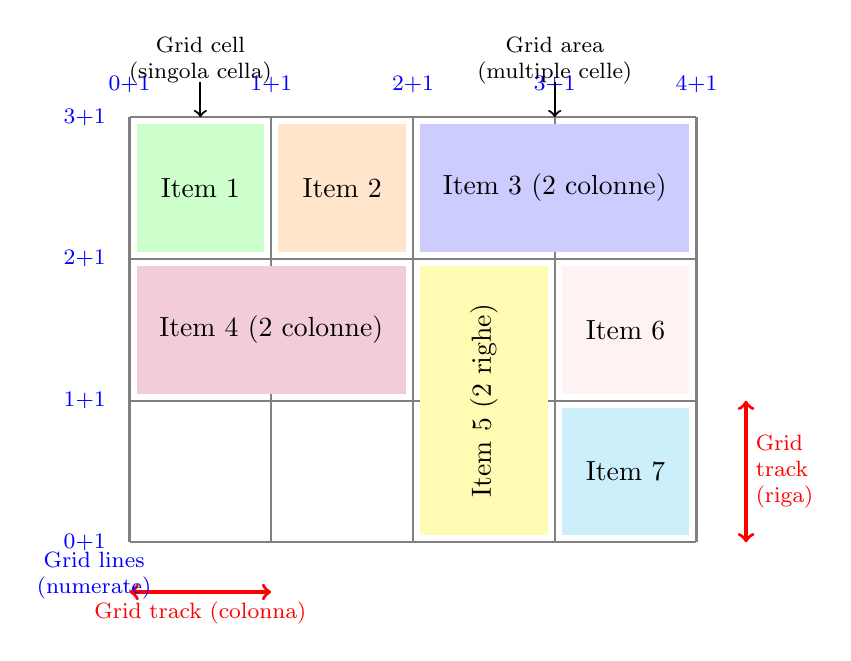
\begin{tikzpicture}[scale=0.9]
    % Grid lines (numerazione)
    \foreach \x in {0,1,2,3,4} {
        \draw[thick, gray] (\x*2,0) -- (\x*2,6);
        \node[above, font=\footnotesize, blue] at (\x*2,6.2) {\x+1};
    }
    \foreach \y in {0,1,2,3} {
        \draw[thick, gray] (0,\y*2) -- (8,\y*2);
        \node[left, font=\footnotesize, blue] at (-0.2,\y*2) {\y+1};
    }

    % Grid cells con contenuto
    \fill[green!20] (0.1,4.1) rectangle (1.9,5.9);
    \node at (1,5) {Item 1};

    \fill[orange!20] (2.1,4.1) rectangle (3.9,5.9);
    \node at (3,5) {Item 2};

    \fill[blue!20] (4.1,4.1) rectangle (7.9,5.9);
    \node at (6,5) {Item 3 (2 colonne)};

    \fill[purple!20] (0.1,2.1) rectangle (3.9,3.9);
    \node at (2,3) {Item 4 (2 colonne)};

    \fill[yellow!30] (4.1,0.1) rectangle (5.9,3.9);
    \node[rotate=90] at (5,2) {Item 5 (2 righe)};

    \fill[pink!20] (6.1,2.1) rectangle (7.9,3.9);
    \node at (7,3) {Item 6};

    \fill[cyan!20] (6.1,0.1) rectangle (7.9,1.9);
    \node at (7,1) {Item 7};

    % Annotazioni
    \draw[<->, red, very thick] (0,-0.7) -- (2,-0.7);
    \node[below, font=\footnotesize, red] at (1,-0.7) {Grid track (colonna)};

    \draw[<->, red, very thick] (8.7,0) -- (8.7,2);
    \node[right, font=\footnotesize, red, align=left] at (8.7,1) {Grid\\track\\(riga)};

    \node[font=\footnotesize, align=center] at (1,6.8) {Grid cell\\(singola cella)};
    \draw[->, thick] (1,6.5) -- (1,6);

    \node[font=\footnotesize, align=center] at (6,6.8) {Grid area\\(multiple celle)};
    \draw[->, thick] (6,6.5) -- (6,6);

    % Legenda grid lines
    \node[below, font=\footnotesize, blue, align=center] at (-0.5,0) {Grid lines\\(numerate)};
\end{tikzpicture}
\end{center}

\begin{tcolorbox}[colback=blue!10, colframe=blue!60, title=Terminologia Grid Visuale]
\begin{itemize}
    \item \textbf{Grid lines}: Linee divisorie numerate (colonna 1, 2, 3, 4, 5 e riga 1, 2, 3, 4)
    \item \textbf{Grid track}: Spazio tra due linee consecutive (colonna o riga)
    \item \textbf{Grid cell}: Singola cella (es: Item 1, Item 2)
    \item \textbf{Grid area}: Area che occupa più celle (es: Item 3 occupa 2 colonne, Item 5 occupa 2 righe)
\end{itemize}
\end{tcolorbox}

\subsubsection{Grid con Template Areas}

\begin{center}
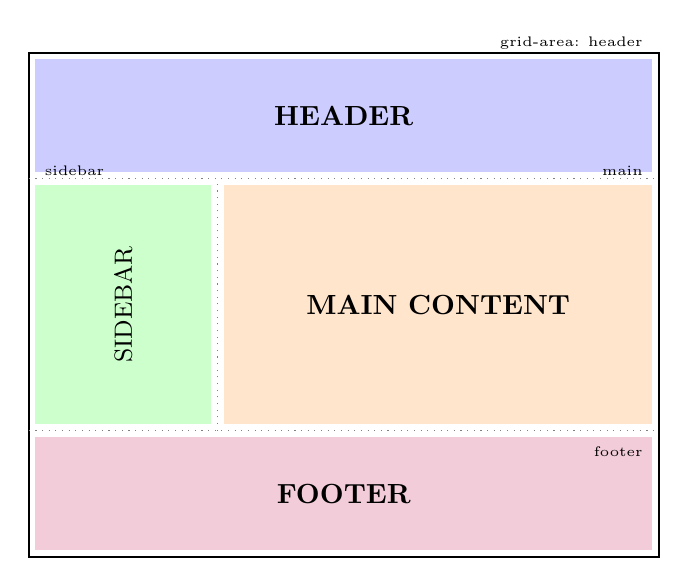
\begin{tikzpicture}[scale=0.8]
    % Disegna la grid
    \draw[thick] (0,0) rectangle (10,8);

    % Header (area header)
    \fill[blue!20] (0.1,6.1) rectangle (9.9,7.9);
    \node[font=\bfseries] at (5,7) {HEADER};
    \node[above left, font=\tiny] at (9.9,7.9) {grid-area: header};

    % Sidebar (area sidebar)
    \fill[green!20] (0.1,2.1) rectangle (2.9,5.9);
    \node[font=\small, rotate=90] at (1.5,4) {SIDEBAR};
    \node[above right, font=\tiny] at (0.1,5.9) {sidebar};

    % Main (area main)
    \fill[orange!20] (3.1,2.1) rectangle (9.9,5.9);
    \node[font=\bfseries] at (6.5,4) {MAIN CONTENT};
    \node[above left, font=\tiny] at (9.9,5.9) {main};

    % Footer (area footer)
    \fill[purple!20] (0.1,0.1) rectangle (9.9,1.9);
    \node[font=\bfseries] at (5,1) {FOOTER};
    \node[below left, font=\tiny] at (9.9,1.9) {footer};

    % Grid lines
    \draw[dotted, gray] (0,6) -- (10,6);
    \draw[dotted, gray] (0,2) -- (10,2);
    \draw[dotted, gray] (3,2) -- (3,6);
\end{tikzpicture}
\end{center}

\begin{lstlisting}[language=CSS]
.container {
  display: grid;
  grid-template-columns: 200px 1fr 1fr 1fr;
  grid-template-rows: auto 1fr auto;
  grid-template-areas:
    "header header header header"
    "sidebar main main main"
    "footer footer footer footer";
}

.header  { grid-area: header; }
.sidebar { grid-area: sidebar; }
.main    { grid-area: main; }
.footer  { grid-area: footer; }
\end{lstlisting}

\begin{nota}
\texttt{grid-template-areas} permette di nominare aree della grid e posizionare elementi semanticamente. Ogni stringa rappresenta una riga, ogni nome ripetuto estende l'area. Usa \texttt{.} (punto) per celle vuote.
\end{nota}

\subsection{Proprietà del Grid Container}

\subsubsection{1. display}

\begin{lstlisting}[language=CSS]
.container {
  display: grid;        /* Block-level grid */
  display: inline-grid; /* Inline-level grid */
}
\end{lstlisting}

\subsubsection{2. grid-template-columns/rows}

Definisce dimensioni colonne e righe:

\begin{lstlisting}[language=CSS]
.container {
  /* 3 colonne: 200px, 1fr, 2fr */
  grid-template-columns: 200px 1fr 2fr;

  /* 3 righe: auto, 300px, auto */
  grid-template-rows: auto 300px auto;

  /* Ripeti pattern: 4 colonne uguali */
  grid-template-columns: repeat(4, 1fr);

  /* Auto-fill responsive */
  grid-template-columns: repeat(auto-fill, minmax(200px, 1fr));
}
\end{lstlisting}

\textbf{Unità di misura}:
\begin{itemize}
  \item \texttt{px, \%, em, rem}: Unità fisse o relative
  \item \texttt{fr}: Frazione dello spazio disponibile (flessibile)
  \item \texttt{auto}: Dimensione basata su contenuto
  \item \texttt{minmax(min, max)}: Range di dimensioni
  \item \texttt{min-content, max-content}: Basato su contenuto
\end{itemize}

\subsubsection{3. grid-template-areas}

Definisce aree nominate:

\begin{lstlisting}[language=CSS]
.container {
  display: grid;
  grid-template-columns: 200px 1fr 200px;
  grid-template-rows: auto 1fr auto;
  grid-template-areas:
    "header header  header"
    "sidebar main   ads"
    "footer footer  footer";
}

.header  { grid-area: header; }
.sidebar { grid-area: sidebar; }
.main    { grid-area: main; }
.ads     { grid-area: ads; }
.footer  { grid-area: footer; }
\end{lstlisting}

\begin{nota}
\texttt{grid-template-areas} rende il codice molto leggibile e mantenibile. Puoi "vedere" il layout nel CSS.
\end{nota}

\subsubsection{4. gap}

Spazio tra righe e colonne:

\begin{lstlisting}[language=CSS]
.container {
  gap: 20px;           /* row-gap e column-gap uguali */
  gap: 20px 10px;      /* row-gap column-gap */
  row-gap: 20px;
  column-gap: 10px;
}
\end{lstlisting}

\subsubsection{5. justify-items / align-items}

Allineamento elementi dentro celle:

\begin{lstlisting}[language=CSS]
.container {
  /* Allineamento orizzontale */
  justify-items: start | end | center | stretch;

  /* Allineamento verticale */
  align-items: start | end | center | stretch;
}
\end{lstlisting}

\subsubsection{6. justify-content / align-content}

Allineamento griglia dentro container:

\begin{lstlisting}[language=CSS]
.container {
  width: 100%;
  height: 100vh;

  /* Allinea griglia orizzontalmente */
  justify-content: start | end | center | space-between | space-around;

  /* Allinea griglia verticalmente */
  align-content: start | end | center | space-between | space-around;
}
\end{lstlisting}

\subsection{Proprietà dei Grid Items}

\subsubsection{1. grid-column / grid-row}

Posizionamento esplicito:

\begin{lstlisting}[language=CSS]
.item {
  /* Colonne da linea 1 a 3 (occupa 2 colonne) */
  grid-column: 1 / 3;
  grid-column-start: 1;
  grid-column-end: 3;

  /* Righe da linea 2 a 4 */
  grid-row: 2 / 4;

  /* Span syntax: occupa 2 colonne */
  grid-column: span 2;

  /* Combinato */
  grid-column: 1 / span 2; /* Inizia a 1, occupa 2 */
}
\end{lstlisting}

\subsubsection{2. grid-area}

Shorthand per posizionamento:

\begin{lstlisting}[language=CSS]
.item {
  /* grid-row-start / grid-column-start / grid-row-end / grid-column-end */
  grid-area: 1 / 1 / 3 / 4;

  /* Oppure usa nome area */
  grid-area: header;
}
\end{lstlisting}

\subsubsection{3. justify-self / align-self}

Override allineamento per singolo elemento:

\begin{lstlisting}[language=CSS]
.special-item {
  justify-self: center; /* Orizzontale */
  align-self: end;      /* Verticale */
}
\end{lstlisting}

\subsection{Esempi Pratici Grid}

\subsubsection{Esempio 1: Layout Pagina Completo}

\begin{lstlisting}[language=HTML]
<div class="page-layout">
  <header>Header</header>
  <nav>Navigation</nav>
  <main>Main Content</main>
  <aside>Sidebar</aside>
  <footer>Footer</footer>
</div>
\end{lstlisting}

\begin{lstlisting}[language=CSS]
.page-layout {
  display: grid;
  grid-template-columns: 200px 1fr 250px;
  grid-template-rows: auto 1fr auto;
  grid-template-areas:
    "header  header  header"
    "nav     main    aside"
    "footer  footer  footer";
  gap: 20px;
  height: 100vh;
}

header { grid-area: header; background: #333; color: white; padding: 1rem; }
nav    { grid-area: nav; background: #f0f0f0; padding: 1rem; }
main   { grid-area: main; background: white; padding: 2rem; }
aside  { grid-area: aside; background: #f9f9f9; padding: 1rem; }
footer { grid-area: footer; background: #333; color: white; padding: 1rem; }

@media (max-width: 768px) {
  .page-layout {
    grid-template-columns: 1fr;
    grid-template-areas:
      "header"
      "nav"
      "main"
      "aside"
      "footer";
  }
}
\end{lstlisting}

\subsubsection{Esempio 2: Gallery Responsive}

\begin{lstlisting}[language=CSS]
.gallery {
  display: grid;
  grid-template-columns: repeat(auto-fill, minmax(250px, 1fr));
  gap: 20px;
  padding: 20px;
}

.gallery img {
  width: 100%;
  height: 250px;
  object-fit: cover;
  border-radius: 8px;
}
\end{lstlisting}

\textbf{Spiegazione \texttt{auto-fill}}:
Il valore \texttt{auto-fill} crea automaticamente tante colonne quante riescono a entrare nel container, rispettando la dimensione minima di 250px. La funzione \texttt{minmax(250px, 1fr)} definisce che ogni colonna deve avere una larghezza compresa tra 250px (minimo) e 1fr (massimo), permettendo alle colonne di espandersi in modo flessibile. Il risultato finale è una gallery completamente responsive che si adatta automaticamente a diverse dimensioni di schermo senza bisogno di media queries.

\subsubsection{Esempio 3: Dashboard Card Layout}

\begin{lstlisting}[language=CSS]
.dashboard {
  display: grid;
  grid-template-columns: repeat(4, 1fr);
  grid-template-rows: repeat(3, 200px);
  gap: 20px;
}

.card-large {
  grid-column: span 2;
  grid-row: span 2;
}

.card-wide {
  grid-column: span 2;
}

.card-tall {
  grid-row: span 2;
}
\end{lstlisting}

\section{Flexbox vs Grid: Quando Usarli}

\begin{table}[h]
\centering
\begin{tabular}{|p{5cm}|p{5cm}|}
\hline
\textbf{Flexbox} & \textbf{Grid} \\
\hline
Layout monodimensionale (riga o colonna) & Layout bidimensionale (righe e colonne) \\
\hline
Componenti UI (navbar, menu, card) & Layout pagina completa \\
\hline
Distribuzione spazio dinamica & Posizionamento esplicito elementi \\
\hline
Allineamento semplice & Sovrapposizione elementi possibile \\
\hline
Crescita/riduzione flessibile & Griglia fissa o responsive \\
\hline
Content-first (dimensione da contenuto) & Layout-first (struttura predefinita) \\
\hline
\end{tabular}
\caption{Confronto Flexbox vs CSS Grid}
\end{table}

\subsection{Quando Usare Flexbox}

\begin{itemize}
  \item Navbar orizzontale o verticale
  \item Allineamento elementi in fila
  \item Centrare elementi (orizzontale/verticale)
  \item Card con altezza uguale
  \item Form con label e input allineati
  \item Footer con elementi distribuiti
\end{itemize}

\subsection{Quando Usare Grid}

\begin{itemize}
  \item Layout pagina completo (header, sidebar, main, footer)
  \item Gallery di immagini
  \item Dashboard con card di dimensioni diverse
  \item Griglia prodotti e-commerce
  \item Calendario o tabella
  \item Magazine-style layout
\end{itemize}

\subsection{Combinazione Flexbox + Grid}

Spesso si usano insieme:

\begin{lstlisting}[language=CSS]
/* Grid per layout pagina */
.page {
  display: grid;
  grid-template-areas: "header" "main" "footer";
}

/* Flexbox per navbar dentro header */
.header {
  display: flex;
  justify-content: space-between;
  align-items: center;
}

/* Grid per gallery dentro main */
.gallery {
  display: grid;
  grid-template-columns: repeat(auto-fill, minmax(200px, 1fr));
}
\end{lstlisting}

\section{Funzioni CSS Avanzate per Grid}

\subsection{repeat()}

\begin{lstlisting}[language=CSS]
/* 4 colonne uguali */
grid-template-columns: repeat(4, 1fr);

/* Equivalente a: */
grid-template-columns: 1fr 1fr 1fr 1fr;

/* Ripeti pattern complesso */
grid-template-columns: repeat(2, 100px 1fr);
/* Risultato: 100px 1fr 100px 1fr */
\end{lstlisting}

\subsection{minmax()}

\begin{lstlisting}[language=CSS]
/* Colonne tra 200px e 400px */
grid-template-columns: repeat(3, minmax(200px, 400px));

/* Responsive: minimo 250px, massimo 1fr (flessibile) */
grid-template-columns: repeat(auto-fill, minmax(250px, 1fr));
\end{lstlisting}

\subsection{auto-fill vs auto-fit}

\begin{lstlisting}[language=CSS]
/* auto-fill: Crea celle extra vuote se c'è spazio */
grid-template-columns: repeat(auto-fill, minmax(200px, 1fr));

/* auto-fit: Espande celle esistenti per riempire spazio */
grid-template-columns: repeat(auto-fit, minmax(200px, 1fr));
\end{lstlisting}

\textbf{Differenza}:
La distinzione tra \texttt{auto-fill} e \texttt{auto-fit} si manifesta nel comportamento quando c'è spazio extra disponibile. Con \texttt{auto-fill}, se hai 3 elementi su uno schermo largo, verranno create 3 colonne per gli elementi più eventuali celle vuote per riempire lo spazio rimanente, mantenendo la griglia completa. Al contrario, con \texttt{auto-fit}, gli stessi 3 elementi verranno espansi per occupare il 100\% dello spazio disponibile, collassando le celle vuote e permettendo agli elementi di crescere fino a riempire completamente il container.

\section{Esercizi}

\subsection{Esercizio 1 (Base): Navbar Flexbox}

Crea una navbar usando Flexbox con:
\begin{itemize}
  \item Logo a sinistra
  \item Menu con link centrati
  \item Pulsante "Login" a destra
  \item Allineamento verticale centrato
  \item Gap 2rem tra elementi menu
\end{itemize}

\subsection{Esercizio 2 (Base): Card Layout Flexbox}

Crea un container con 4 card usando Flexbox:
\begin{itemize}
  \item Card con altezza uguale
  \item Wrapping su mobile (max-width 768px)
  \item Gap 20px tra card
  \item Ogni card con flex-basis 300px
\end{itemize}

\subsection{Esercizio 3 (Intermedio): Griglia Prodotti Grid}

Crea una griglia 3x3 di prodotti usando CSS Grid:
\begin{itemize}
  \item 3 colonne uguali su desktop
  \item 2 colonne su tablet (max 1024px)
  \item 1 colonna su mobile (max 768px)
  \item Gap 20px
  \item Un prodotto "featured" che occupa 2 colonne
\end{itemize}

\subsection{Esercizio 4 (Intermedio): Dashboard Layout}

Crea un dashboard usando Grid con:
\begin{itemize}
  \item Header full-width (grid-column: 1 / -1)
  \item Sidebar sinistra 250px
  \item Main content area (1fr)
  \item Widget area destra 300px
  \item Footer full-width
  \item Altezza totale 100vh
\end{itemize}

\subsection{Esercizio 5 (Avanzato): Layout Magazine}

Crea un layout magazine-style con Grid:
\begin{itemize}
  \item 1 articolo grande (2 colonne × 2 righe)
  \item 4 articoli medi (1 colonna × 1 riga)
  \item Responsive: mobile 1 colonna, tablet 2 colonne, desktop 4 colonne
  \item Usa \texttt{grid-template-areas}
\end{itemize}

\subsection{Esercizio 6 (Avanzato): Gallery Responsive Auto}

Crea una gallery completamente responsive usando:
\begin{itemize}
  \item \texttt{grid-template-columns: repeat(auto-fit, minmax(250px, 1fr))}
  \item Aspect ratio 1:1 per immagini
  \item Hover effect: scale(1.05)
  \item Gap 15px
  \item Nessuna media query richiesta
\end{itemize}

\subsection{Esercizio 7 (Avanzato): Combinazione Flexbox + Grid}

Crea una pagina completa combinando Flexbox e Grid:
\begin{itemize}
  \item Grid per layout pagina (header, main, footer)
  \item Flexbox per navbar dentro header
  \item Grid per gallery prodotti dentro main
  \item Flexbox per footer con 3 sezioni distribuite
  \item Responsive su mobile: tutto verticale
\end{itemize}

\section{Best Practices}

\subsection{Flexbox}

\begin{itemize}
  \item Usa \texttt{flex} shorthand invece di grow/shrink/basis separati
  \item Usa \texttt{gap} invece di margin per spaziatura
  \item Mobile-first: \texttt{flex-direction: column} su mobile, \texttt{row} su desktop
  \item Evita \texttt{justify-content: space-between} con numero variabile elementi
  \item Per centramento: \texttt{justify-content: center; align-items: center;}
\end{itemize}

\subsection{Grid}

\begin{itemize}
  \item Usa \texttt{fr} per layout flessibili, \texttt{px} per dimensioni fisse
  \item Preferisci \texttt{grid-template-areas} per layout complessi (leggibilità)
  \item Usa \texttt{auto-fit/auto-fill} per gallery responsive senza media queries
  \item Definisci grid gap a livello container, non margin su item
  \item Nomina le grid lines per posizionamento più chiaro
\end{itemize}

\subsection{Generale}

\begin{itemize}
  \item Flexbox per componenti, Grid per layout
  \item Combina i due sistemi quando necessario
  \item Testa su browser diversi (supporto IE11 limitato)
  \item Usa CSS Grid per overlay/sovrapposizione elementi
  \item Mobile-first: layout semplice su mobile, complesso su desktop
\end{itemize}

\section{Supporto Browser}

\begin{itemize}
  \item \textbf{Flexbox}: Supportato da IE11+, tutti i browser moderni
  \item \textbf{Grid}: Supportato da IE11 (con prefissi -ms-), tutti i browser moderni
  \item \textbf{gap in Flexbox}: Chrome 84+, Firefox 63+, Safari 14.1+ (2021)
  \item \textbf{Fallback}: Usa feature queries \texttt{@supports}
\end{itemize}

\begin{lstlisting}[language=CSS]
/* Fallback per browser senza grid */
.container {
  display: flex; /* Fallback */
}

@supports (display: grid) {
  .container {
    display: grid;
    grid-template-columns: repeat(3, 1fr);
  }
}
\end{lstlisting}

\section{Risorse Utili}

\begin{itemize}
  \item \textbf{Flexbox Froggy}: \url{https://flexboxfroggy.com/} (gioco interattivo)
  \item \textbf{Grid Garden}: \url{https://cssgridgarden.com/}
  \item \textbf{CSS-Tricks Flexbox Guide}: \url{https://css-tricks.com/snippets/css/a-guide-to-flexbox/}
  \item \textbf{CSS-Tricks Grid Guide}: \url{https://css-tricks.com/snippets/css/complete-guide-grid/}
  \item \textbf{MDN Flexbox}: \url{https://developer.mozilla.org/en-US/docs/Web/CSS/CSS_Flexible_Box_Layout}
  \item \textbf{MDN Grid}: \url{https://developer.mozilla.org/en-US/docs/Web/CSS/CSS_Grid_Layout}
\end{itemize}

\section{Riepilogo}

\subsection{Flexbox}

\begin{itemize}
  \item Layout monodimensionale (riga o colonna)
  \item Proprietà container: display, flex-direction, flex-wrap, justify-content, align-items, align-content, gap
  \item Proprietà item: flex-grow, flex-shrink, flex-basis, flex (shorthand), order, align-self
  \item Perfetto per navbar, card, allineamenti semplici
  \item \texttt{justify-content}: asse principale, \texttt{align-items}: asse trasversale
\end{itemize}

\subsection{Grid}

\begin{itemize}
  \item Layout bidimensionale (righe e colonne)
  \item Proprietà container: display, grid-template-columns/rows, grid-template-areas, gap, justify/align-items, justify/align-content
  \item Proprietà item: grid-column/row, grid-area, justify/align-self
  \item Funzioni: repeat(), minmax(), auto-fill, auto-fit
  \item Perfetto per layout pagina, gallery, dashboard
  \item \texttt{fr}: frazione spazio disponibile
\end{itemize}

\subsection{Quando Usare}

\begin{itemize}
  \item \textbf{Flexbox}: Componenti UI, allineamento monodimensionale, distribuzione spazio
  \item \textbf{Grid}: Layout completi, posizionamento bidimensionale, griglie
  \item \textbf{Insieme}: Grid per struttura pagina + Flexbox per componenti interni
\end{itemize}
